% =============================================================================
% s71_c0_results.tex --- Draft for main.tex §7.1: the reliability x
% recoverability decision surface (C0 results paragraph).
%
% SERVES: Claim C0 (reliability x recoverability decision surface, motivation
%   chapter), levers C0.1 (reliability axis: per-dimension x severity diagnostic
%   AUC grid) and C0.2 (recoverability axis: can enhancement rescue the
%   diagnosis; bridges C1 and C3). Target location: §7.1, story arc §7.1.
%
% DATA SOURCE (verifier PASS, 0 drift, do not edit numbers without re-verifying):
%   results/c0_decision_surface.csv -- 25 rows = 5 axes x 5 severity levels,
%   n=360 / cell, bootstrap 2000-sample 95% CI. AUC-led main axis;
%   recoverability_delta = auc_enhanced - auc with bootstrap 95% CI.
%
% C3 WORDING SAFEGUARD (mandatory, STORY "C0 decision surface" block):
%   Do NOT generalise to "enhancement is unsafe under severe degradation".
%   Only contrast S5 shows a significant HURT; blur S5 and color_shift S5 still
%   benefit. The contrast-S5 cell is a per-DIMENSION supplementary trigger for
%   query-for-retake; it does NOT replace and is NOT conflated with the
%   per-CLASS E5/E6 evidence (§7.4 / §7.8).
% =============================================================================

\subsection{The Reliability\,$\times$\,Recoverability Decision Surface}
\label{sec:exp-surface}

We chart a \emph{reliability\,$\times$\,recoverability decision surface} over a
$5\times5$ grid that crosses our five degradation dimensions (blur, brightness,
completeness, colour shift, contrast) with five severity levels each, with
$n=360$ images per cell and bootstrap $2000$-sample $95\%$ confidence intervals
throughout. The primary (reliability) axis reports diagnostic AUC under
degradation; a second (recoverability) axis reports the change in AUC once the
enhancer is applied, $\Delta_{\text{rec}} = \mathrm{AUC}_{\text{enh}} -
\mathrm{AUC}$, so that each cell answers two questions at once: \emph{how much
does this corruption cost diagnosis}, and \emph{can enhancement buy it back}.
This per-dimension $\times$ per-severity, AUC-led view is complementary to, and
deliberately distinct from, the per-dimension expected-calibration-error /
QCTS analysis of \citet{ANON-BMVC} (Tab.~\texttt{perdeg} there, cited but not
reproduced), which neither sweeps severity nor includes completeness, and which
carries no recoverability axis. The full grid is plotted as a heatmap in
\cref{fig:c0-surface}; we summarise the two axes below.

\begin{figure}[t]
  \centering
  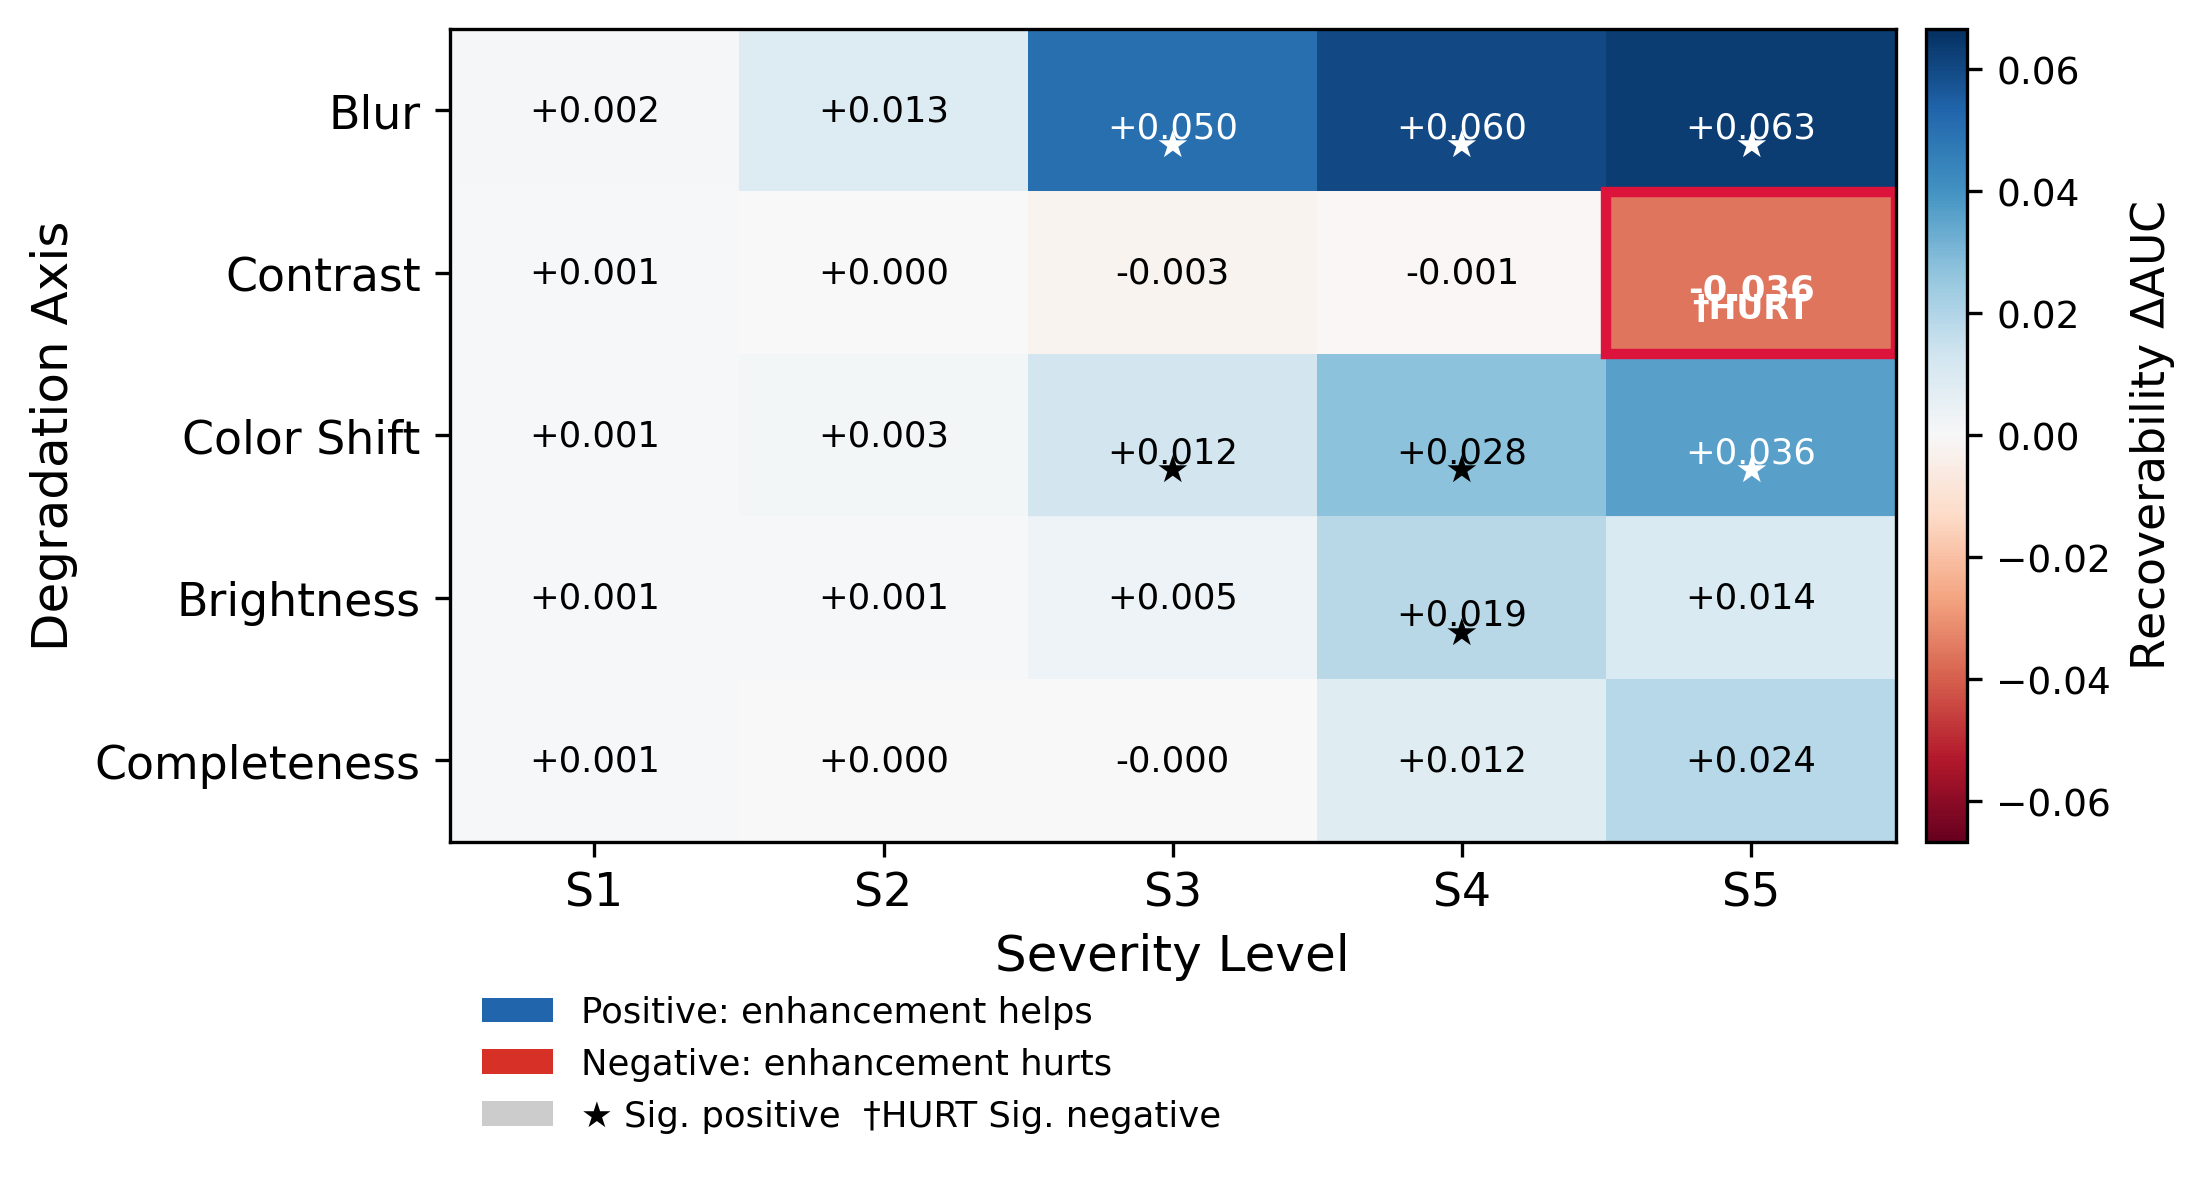
\includegraphics[width=0.92\linewidth]{figures/c0_recoverability_heatmap.pdf}
  \caption{\textbf{Reliability\,$\times$\,recoverability decision surface.} Per-cell
  recoverability $\Delta\mathrm{AUC}=\mathrm{AUC}_{\text{enh}}-\mathrm{AUC}_{\text{deg}}$
  across five degradation dimensions (rows) and five severity levels S1--S5 (columns),
  $n=360$/cell. Blue cells (positive) are where enhancement recovers diagnosis; red cells
  (negative) are where it hurts. Significant cells (bootstrap $95\%$ CI excluding zero) are
  starred ($\star$ recovers) or marked $\dagger$HURT (harms); the single harmful cell is
  contrast at S5 ($\Delta=-0.0355$, CI $[-0.0783,-0.0013]$). Blur and colour-shift recover
  significantly from S3 onward, whereas completeness stays statistically indistinguishable
  from zero throughout.}
  \label{fig:c0-surface}
\end{figure}

\paragraph{Reliability axis.}
Diagnostic AUC degrades monotonically, or near-monotonically, with severity
along every dimension (\cref{fig:c0-reliability}), but the magnitude differs sharply by corruption type.
Ranking the drop from the identity anchor (S1) to the most severe level (S5),
blur is by far the most fragile: AUC falls from $0.9219$ at S1 to $0.8307$ at S5
($\sigma=3.5$), a strictly monotone decline of $-0.0911$. Completeness is next
($0.9238 \to 0.8722$ at crop ratio $0.515$, $-0.0516$), and rises slightly over
the mild levels ($0.924 \to 0.929$ across S1--S3) before falling. Colour shift
follows ($0.9239 \to 0.8870$ at shift $0.34$, $-0.0369$). The two dimensions
that look most robust on this axis are brightness ($0.9238 \to 0.9061$ at
multiplier $0.345$, only $-0.0177$, non-monotone) and contrast ($0.9238 \to
0.9085$ at $\alpha=0.19$, $-0.0153$). We emphasise that contrast is only
\emph{superficially} robust here: its reliability drop is the smallest of the
five, yet, as the recoverability axis shows next, it is the single dimension on
which enhancement actively backfires at the extreme level. All per-cell AUC
values are reported with bootstrap $95\%$ CIs in \cref{app:surface}.

\begin{figure}[t]
  \centering
  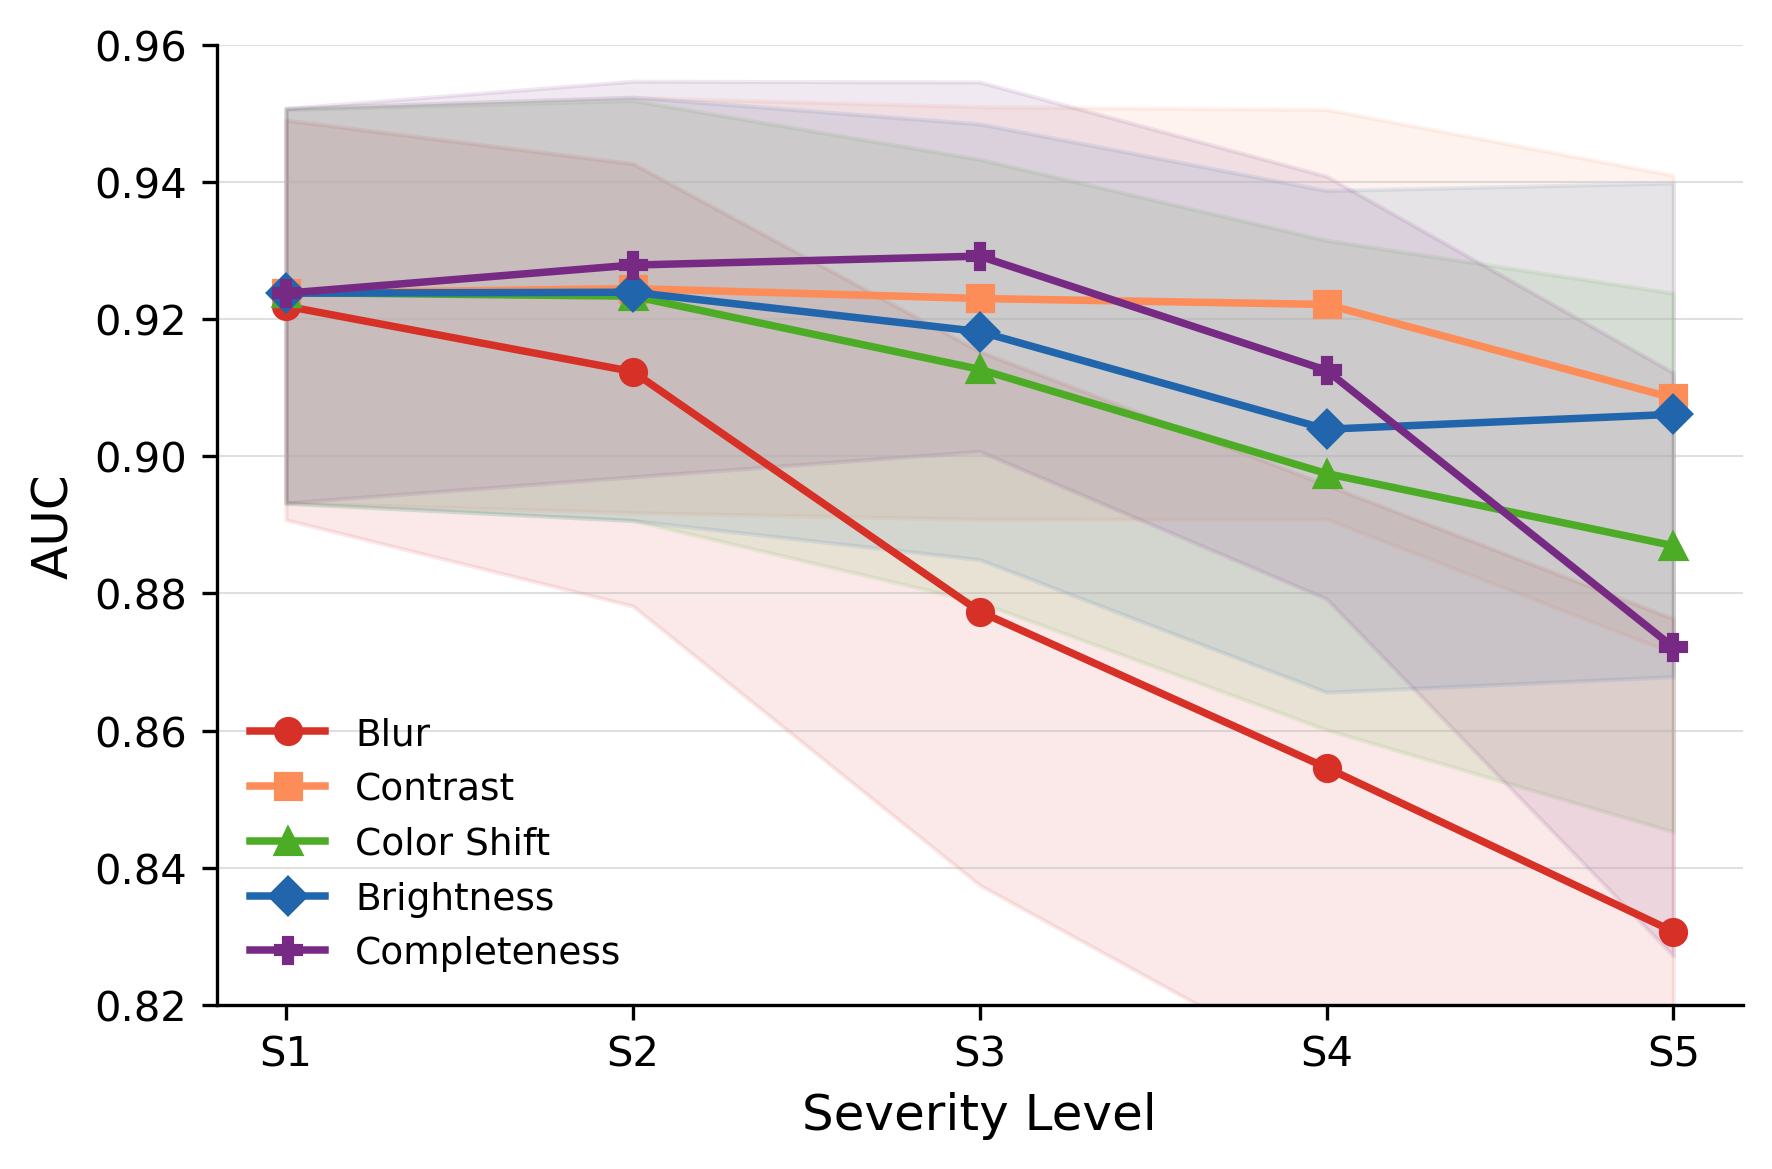
\includegraphics[width=0.82\linewidth]{figures/c0_reliability_curves.pdf}
  \caption{\textbf{Reliability curves: diagnostic AUC versus severity, per degradation
  dimension.} Each curve traces held-out AUC as a single corruption is intensified from the
  identity anchor (S1) to its most severe level (S5), $n=360$/cell (source
  \texttt{results/c0\_decision\_surface.csv}). Blur is the most fragile dimension
  ($0.922\!\to\!0.831$, $-0.091$); contrast and brightness drop least
  ($-0.015$, $-0.018$). The small reliability drop of contrast is deceptive: the
  recoverability surface (\cref{fig:c0-surface}) shows it is the one dimension where
  enhancement actively backfires at S5.}
  \label{fig:c0-reliability}
\end{figure}

\paragraph{Recoverability axis.}
Overlaying $\Delta_{\text{rec}}$ on the same grid separates the surface into
three regimes (a cell is called significant only when its bootstrap $95\%$ CI
excludes zero).
\textbf{(i) Reliably recoverable.} On blur, enhancement significantly restores
diagnosis from severity S3 onward ($\Delta_{\text{rec}} = +0.0500$, $+0.0598$,
$+0.0634$ at S3/S4/S5, all CI lower bounds $>0$); on colour shift it likewise
helps from S3 onward ($+0.0124$, $+0.0275$, $+0.0361$ at S3/S4/S5, all CI lower
bounds $>0$), with the enhanced AUC at S4/S5 returning to $\approx 0.924$ and
thus nearly bridging back to the clean baseline. In both cases the help-vs-hurt
transition occurs at S3.
\textbf{(ii) Uncertain.} Completeness is \emph{partially recoverable} but never
significantly so: all five levels straddle zero (e.g.\ S5
$\Delta_{\text{rec}} = +0.0236$, $95\%$ CI $[-0.0079, +0.0572]$), and brightness
reaches significance at S4 only ($+0.0186$, CI excludes zero) --- consistent
with its being the most reliability-robust axis, where there is little to
recover.
\textbf{(iii) Significantly harmful.} Exactly one cell out of all $25$ shows
enhancement significantly \emph{degrading} diagnosis: contrast at S5
($\alpha=0.19$), where $\Delta_{\text{rec}} = -0.0355$ with $95\%$ CI
$[-0.0783, -0.0013]$ (excludes zero), driving AUC from $0.9085$ down to
$0.8734$ after enhancement.

\paragraph{Reading the surface.}
The surface motivates quality-aware triage directly: most corruptions are both
costly and recoverable (the moderate window that the diagnosis-preserving
enhancer of \cref{sec:enhance} is designed to exploit), but at least one
extreme corruption is recoverable \emph{in name only}, and there enhancement
should be withheld. Concretely, severe contrast loss ($\alpha=0.19$) drives a
significant $-0.0355$ ($95\%$ CI excludes zero) drop in diagnostic AUC after
enhancement, which we treat as one \emph{per-dimension} trigger for the
query-for-retake channel rather than as a reason to enhance. We are deliberately
narrow here: \emph{we do not generalise to ``enhancement is unsafe under severe
degradation''.} At the same S5 severity, blur ($\Delta_{\text{rec}} = +0.0634$)
and colour shift ($+0.0361$) remain significantly beneficial, so severity alone
is not a safe gate --- the gate must be dimension-aware. This contrast-S5 cell
is a supplementary, per-dimension trigger; it does not replace, and should not
be conflated with, the per-class severe-degradation and melanoma-rescue evidence
that drives the safety boundary in \cref{sec:exp-boundary} (E5/E6, reported by
class rather than by dimension). Together the two readings --- a per-dimension
contrast trigger here and a per-class melanoma/severe trigger there --- give the
query-for-retake gate two independent sources of motivation.
